% \chapter{Preliminaries} 
% \label{ch:prelim}



% \begin{chapternotes}
%   This chapter contains material previously published ...
% \end{chapternotes}

\section{Basics}
In the following we will  introduce the topics ... 

This is my text with an example \autoref{fig:example} and example
citation~\cite{Bringhurst1993} or \textcite{Bringhurst1993}. 

\begin{figure}
	\centering
	\includegraphics[width=3cm]{htl_at}
	\caption{Example caption.}
	\label{fig:example}
\end{figure}

Now you are able to write your own document. Always keep in mind: it's
the \emph{content} that matters, not the form. But good typography is
able to deliver the content much better than information set with bad
typography. This template allows you to concentrate on writing good
content while the form is done by the template definitions.

\section{Additional Features}

You can use abbreviations using the \verb+\ac{}+ command like this: \ac{LTL}, 
where the abbreviation is expanded on first use and then printed normally: \ac{LTL}. 

Enumerations
\begin{enumerate}
	\item Foo
	\item Bar
\end{enumerate}

and itemizations
\begin{itemize}
	\item One
	\item Two
	\item Three
\end{itemize}

TikZ Pictures like in \autoref{fig:def:prelim:ltl:kl-loop}
\begin{figure}
  \centering
  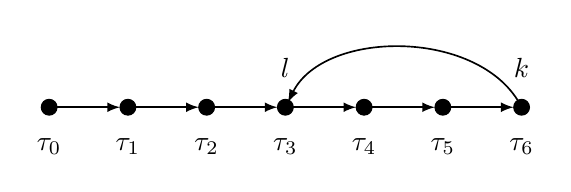
\begin{tikzpicture}
    \foreach \x in {0,1,2,3,4,5,6} 
    \draw[fill] (\x,5.5) circle (0.1);
    \foreach \x in {0,1,2,3,4,5} 
    \draw[-latex,semithick] (\x,5.5) -- +(0.9,0);
    \draw[-latex,shorten >=2,semithick] (6,5.5) .. controls (5.5,6.5) and (3.5,6.5) .. (3,5.5);
    \foreach \x in {0,1,2,3,4,5,6}
    \node at (\x,5) {$\tau_{\x}$};
    % \node at (-0.5,5) {$t=$};
    \node at (6,6) {$k$};
    \node at (3,6) {$l$};
  \end{tikzpicture}
  \caption{Some funny picture}
  \label{fig:def:prelim:ltl:kl-loop}
\end{figure}


Tables: see \autoref{tab:example}.

\begin{table}
	\centering
	\caption{Example Table}
	\label{tab:example}
	\begin{tabular}{llc}
	\toprule
	A & B & C\\
	\midrule
	1 & 2 & unknown\\
	x & y & z\\
	\bottomrule
	\end{tabular}
\end{table}

\begin{todobox}
ToDo: write some more content
\end{todobox}


Now you are able to write your own document. Always keep in mind: it's
the \emph{content} that matters, not the form. But good typography is
able to deliver the content much better than information set with bad
typography. This template allows you to concentrate on writing good
content while the form is done by the template definitions.